

\begin{enumerate}
    \item  Se implementa en lenguaje C una \textit{s-Function} que recibe como entrada una señal digital con tasa de muestro de $16~kps$, cuya salida actualiza cada $20~ms$ el valor RMS de los últimos $20~ms$ transcurridos de la señal.
    
    
    Como se desea calcular RMS para frames de $20~ms$ de una señal de frecuencia de muestreo de $16~kps$, con las conclusiones obtenidas en el apartado 1, se puede determinar cual es el valor de N necesario en el código para poder cumplir con las especificaciones dadas. En este caso
    
    $$Ts = \frac{1}{Fs} = \frac{1}{16~kps} = 62.5~\mu s$$
    
    Luego si se busca  $T = 20~ms$, entonces
    
    $$ N = \frac{T}{Ts}= \frac{20 ~ms}{62.5~\mu s}= 320$$
    
    El código  en donde se implementa la \textit{s-Function mencionada} es el siguiente
    
    
    
    \begin{lstlisting}
//Ts = 1/16kps = 62 us -> N = 20ms/62us = 320
    #define N 320 
    double rms_20ms(double input) {

	static double buffer = 0;
	static unsigned int cont = 0;
	static double output = 0;
    
//eleva la muestra al cuadrado y la guarda en la sumatoria
	buffer = buffer + pow(input,2);

//reinicia el buffer y entrega el rms acumulado 
	if (cont >= N)   
	    {
		buffer = buffer/N;  
		output = sqrt(buffer);
		buffer = 0;
		cont = 0;
    	}
	else
		{
			cont ++;
		}


	return output;
}


    \end{lstlisting}
\end{enumerate}


Al agregar el código asociado a la \textit{s-Function} implementada para esta tarea, procede a simular su funcionamiento utilizando como entrada el archivo de audio \textit{musica\_16\_16.wav} ya que cumple con el requerimiento de frecuencia de muestro de $16~kps$, obteniendo de esta forma la gráfica que se muestra en la figura \ref{envolve}


Las figuras \ref{envolve10ms} y \ref{envolve40ms} intentan evidenciar como cambia la envolvente dependiendo del tamaño del frame que se procesa, siendo en el primer caso de una duración de $10~ms$ y $40~ms$ en  el segundo.

\begin{figure}[H]
    \centering
    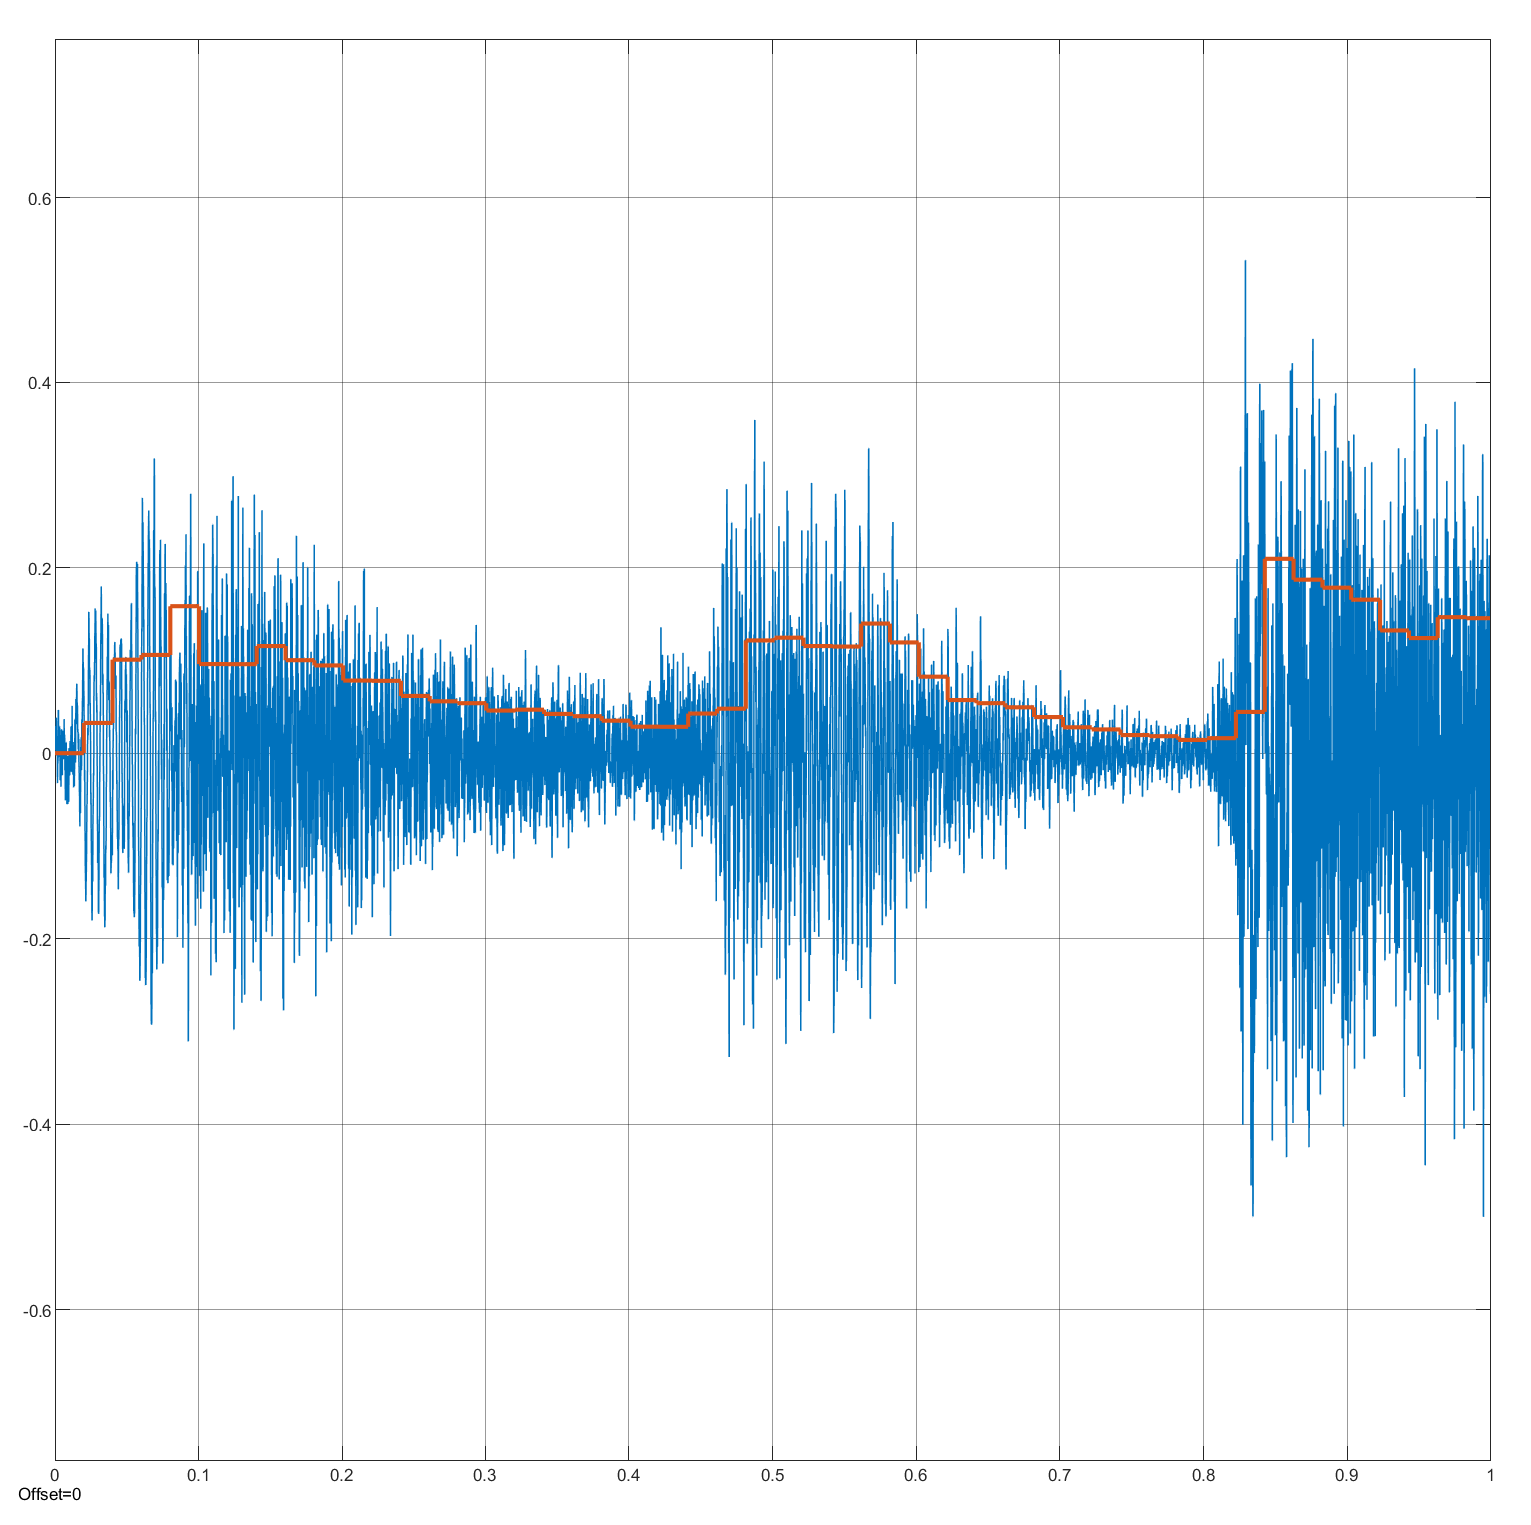
\includegraphics[scale = 0.4]{Figuras/p4_1_envolvente_frame.eps}
    \caption{Resultado de calculo del valor RMS para frames de $20~ms$ al archivo de audio \textit{musica\_16\_16.wav}.}
    \label{envolve}
\end{figure}


\begin{figure}[H]
    \centering
    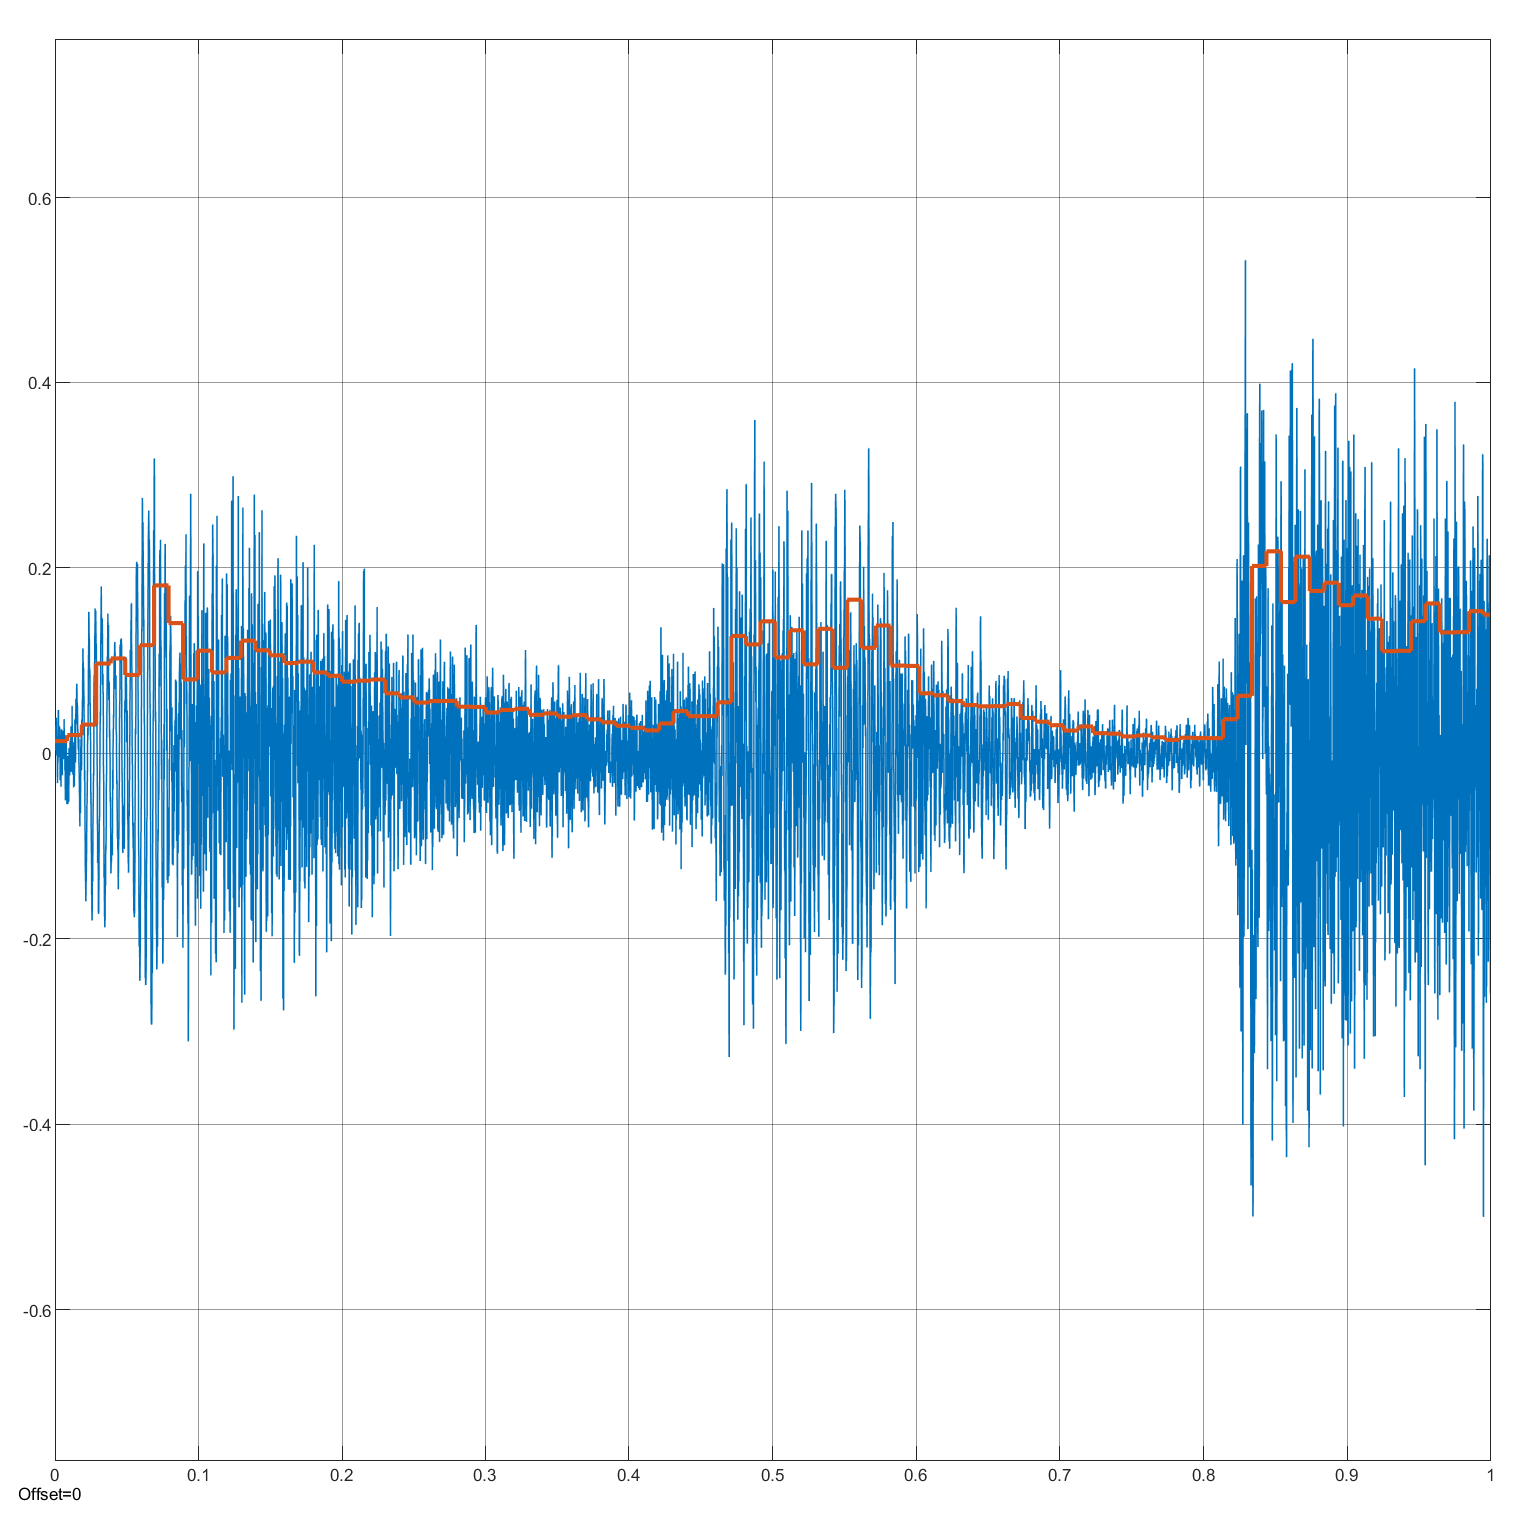
\includegraphics[scale = 0.4]{Figuras/rms_10ms.eps}
    \caption{Resultado de calculo del valor RMS para frames de $10~ms$ al archivo de audio \textit{musica\_16\_16.wav}.}
    \label{envolve10ms}
\end{figure}

\begin{figure}[H]
    \centering
    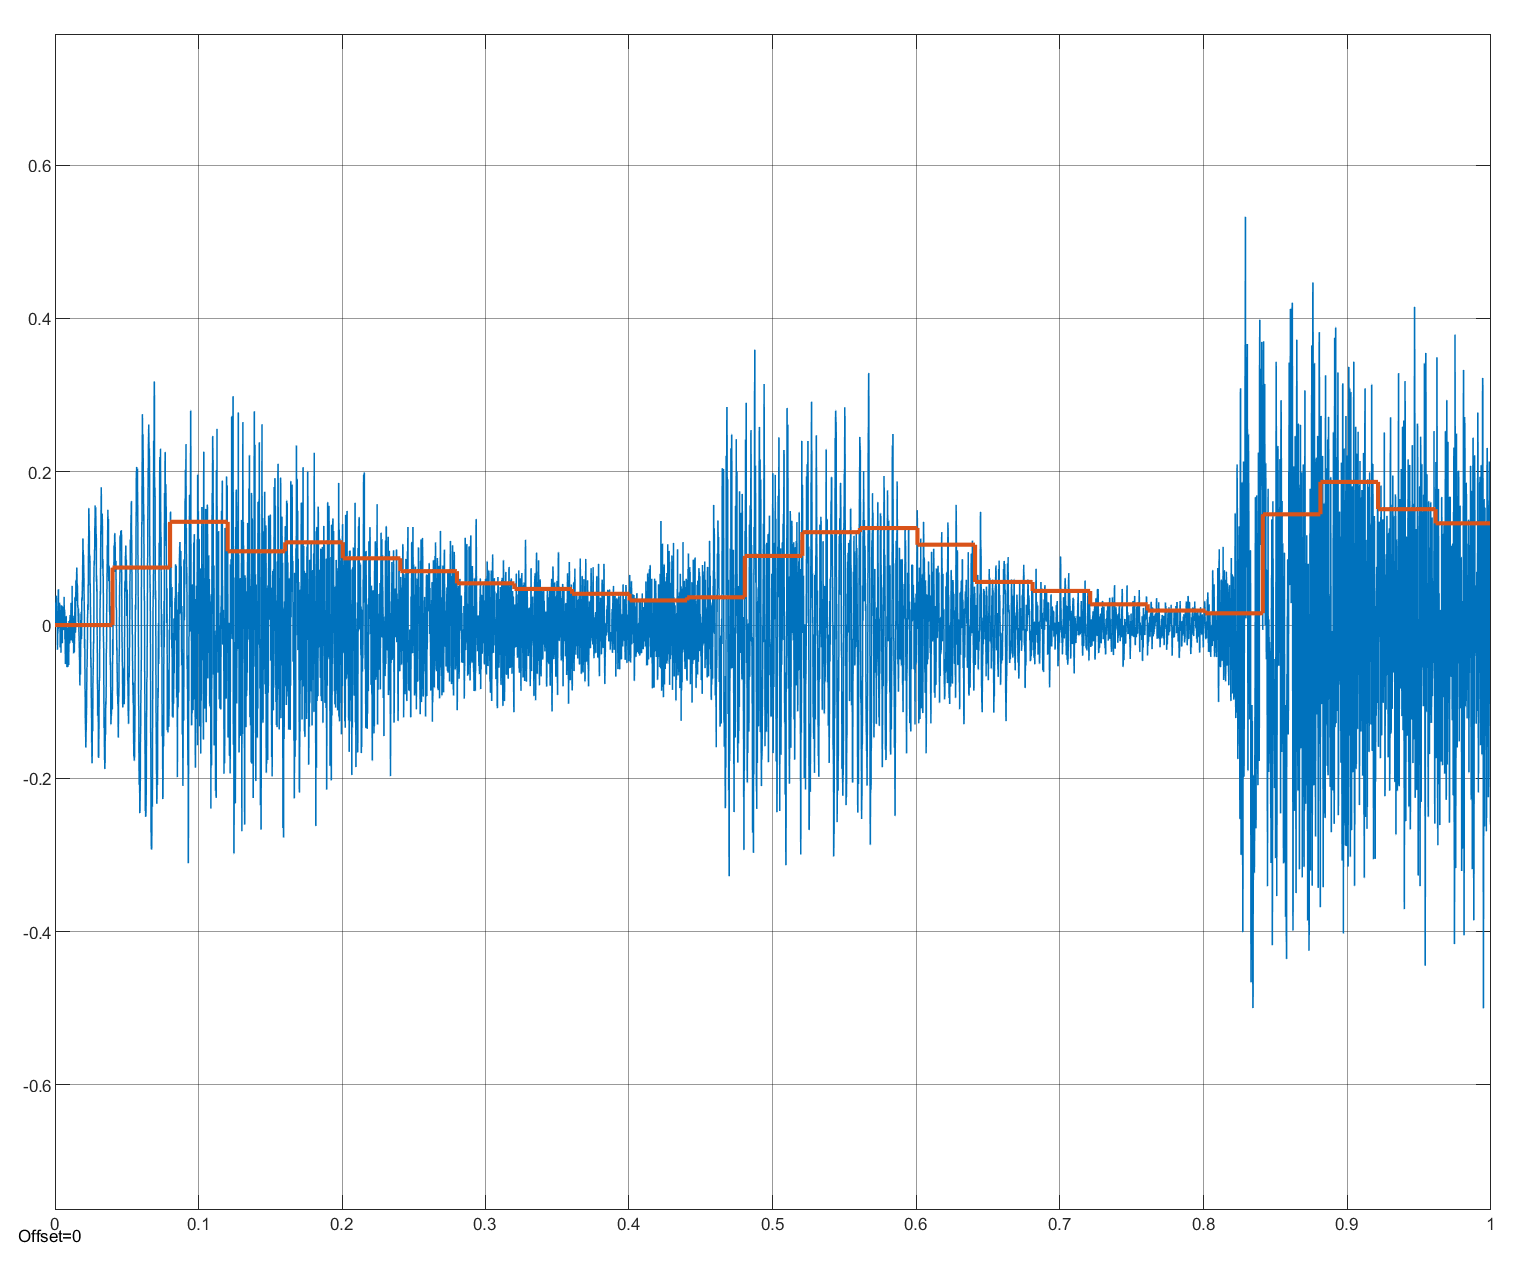
\includegraphics[scale = 0.4]{Figuras/rms40ms.eps}
    \caption{Resultado de calculo del valor RMS para frames de $40~ms$ al archivo de audio \textit{musica\_16\_16.wav}.}
    \label{envolve40ms}
\end{figure}